Most of our system sequence diagrams have been extended to interaction diagrams of system-wide operations. 
An example of this can be seen in figure \ref{fig:merge-ssd}, 
which has laid basis for the interaction diagram depicting the merge process, 
as seen in appendix \ref{sec:interactiondiagrams} on page \pageref{fig:interaction-merge-diagram}
The merge operation (figure \ref{fig:merge-ssd}) is a central feature of the \SOP 
system, so it has been subject to some scrutiny in the documentation.


\begin{figure}[hbt]
	\centering
	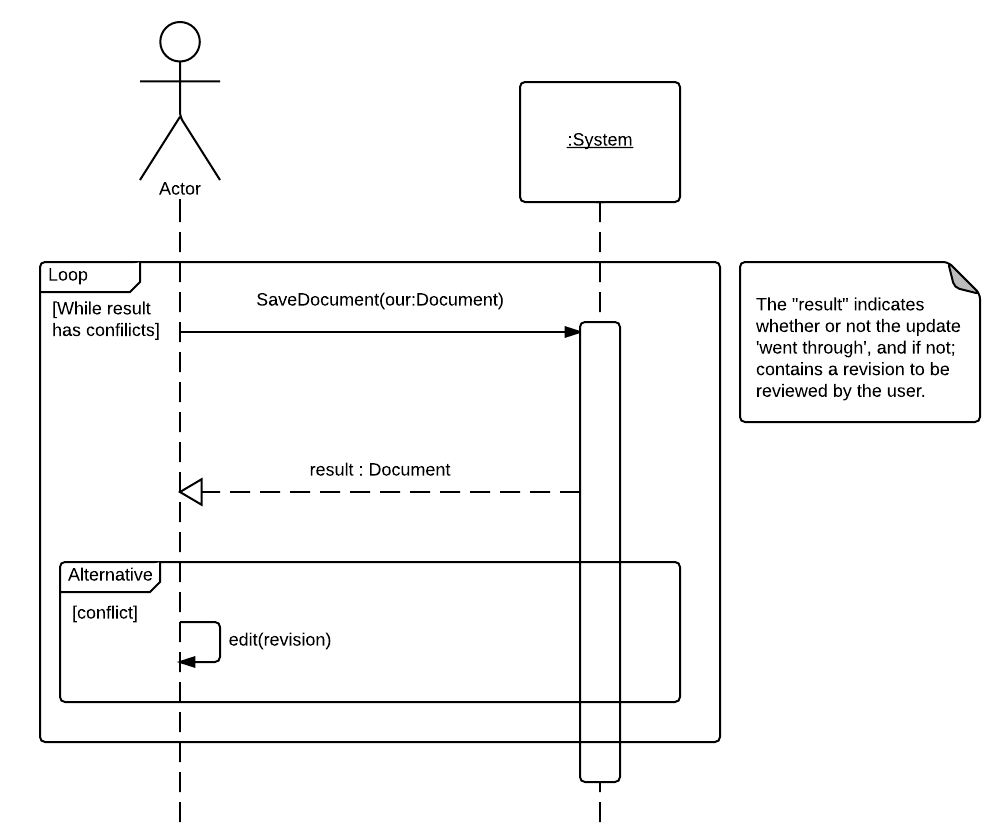
\includegraphics[width=1\textwidth]{Software_analysis/graphics/Merge-ssd.png}
	\caption{A system sequence diagram, depicting the merge process}
	\label{fig:merge-ssd}
\end{figure}
